%% main.tex
%% HVM-Codec IEEE T-ITS manuscript skeleton.
%% Modified from the IEEEtran bare_jrnl.tex journal template.
%% Keep IEEEtran.cls and IEEE publication rules unchanged when preparing the final submission.

\documentclass[journal]{IEEEtran}

% -------------------- Packages --------------------
\usepackage{cite}
\usepackage{amsmath,amssymb}
\usepackage{graphicx}
\usepackage{array}
\usepackage{booktabs}
\usepackage{multirow}
\usepackage[caption=false,font=footnotesize]{subfig}
\usepackage{url}

% -------------------- Project Macros --------------------
\newcommand{\HVM}{HVM-Codec}
\newcommand{\Iseq}{\mathcal{I}}
\newcommand{\Mmem}{\mathcal{M}}
\newcommand{\Kframes}{\mathcal{K}}
\newcommand{\Smotion}{\mathcal{S}}
\newcommand{\Aanchor}{\mathcal{A}}
\newcommand{\Llang}{\mathcal{L}}
\newcommand{\Pprompt}{\mathcal{P}}
\newcommand{\Ihat}{\hat{\mathcal{I}}}

% A compile-safe placeholder for figures before final graphics are ready.
\newcommand{\placeholderfig}[2]{%
\fbox{%
\begin{minipage}[c][#1][c]{#2}
\centering
\vspace{0.2em}
\textbf{Figure Placeholder}\\[0.4em]
Replace this box with the final vector figure or high-resolution image.
\vspace{0.2em}
\end{minipage}}
}

% Correct bad hyphenation here.
\hyphenation{op-tical net-works semi-conduc-tor VSLAM image-text edge-cloud}

\begin{document}

% -------------------- Title --------------------
\title{\HVM: Human-Inspired Image--Text Visual Memory Coding for Edge--Cloud Visual SLAM}

% -------------------- Authors --------------------
% TODO: Replace author names, memberships, affiliations, and funding/manuscript information.
\author{First~Author,~\IEEEmembership{Member,~IEEE,}
        Second~Author,~\IEEEmembership{Member,~IEEE,}
        and~Third~Author,~\IEEEmembership{Senior Member,~IEEE}%
\thanks{This work was supported in part by XXX.}%
\thanks{First Author and Second Author are with XXX University, City, Country (e-mail: author@example.com).}%
\thanks{Third Author is with XXX Laboratory, City, Country.}%
\thanks{Manuscript received XXX; revised XXX.}}

% -------------------- Running Header --------------------
\markboth{IEEE Transactions on Intelligent Transportation Systems}%
{First Author \MakeLowercase{\textit{et al.}}: \HVM: Human-Inspired Image--Text Visual Memory Coding for Edge--Cloud VSLAM}

\maketitle

% -------------------- Abstract --------------------
\begin{abstract}
Edge--cloud visual simultaneous localization and mapping (VSLAM) relies on continuous visual streams, but transmitting dense image sequences from resource-constrained edge devices to cloud-side SLAM backends introduces substantial bandwidth and energy costs. Existing image and video codecs mainly optimize pixel-level fidelity or perceptual quality, which does not necessarily preserve the geometric continuity and trackable structures required by VSLAM. Inspired by human visual memory, this paper proposes \HVM, a human-inspired image--text visual memory coding framework for edge--cloud VSLAM. The edge encoder represents a visual sequence using boundary frames, lightweight motion memories, visual novelty anchors, and compact language conditions. Boundary frames provide geometric constraints, language memories encode high-level motion and semantic priors, and a cloud-side world-model decoder uses its learned visual prior to imagine and reconstruct task-usable intermediate frames. To improve SLAM-friendly reconstruction, the decoder is further fine-tuned with LoRA. The proposed codec is evaluated by downstream VSLAM trajectory quality rather than pixel fidelity alone, including absolute pose error, relative pose error, trajectory completeness, bandwidth reduction, and runtime.
\end{abstract}

% -------------------- Keywords --------------------
\begin{IEEEkeywords}
Edge--cloud VSLAM, image--text coding, visual memory coding, task-oriented compression, world model, generative reconstruction, LoRA fine-tuning.
\end{IEEEkeywords}

\IEEEpeerreviewmaketitle

% !TEX root = ../main.tex

% ==================================================
\section{Introduction}
\label{sec:introduction}
% ==================================================

\IEEEPARstart{V}{isual} simultaneous localization and mapping (VSLAM) enables mobile robots, autonomous platforms, and embodied intelligent systems to estimate motion and build maps from visual observations. With the increasing availability of cloud-side computation, edge--cloud VSLAM has become an attractive paradigm: the edge device captures visual observations with limited onboard resources, while the cloud executes more powerful perception, optimization, and mapping modules. This division, however, shifts a critical burden to the communication link. A monocular or RGB-D camera continuously produces high-frame-rate image streams, and transmitting dense visual data from the edge to the cloud incurs substantial bandwidth, energy, and latency costs. The bottleneck becomes more severe in long-term navigation, large-scale deployment, and bandwidth-constrained wireless environments.

% Suggested Fig. 1: human-inspired concept figure.
\begin{figure}[!t]
\centering
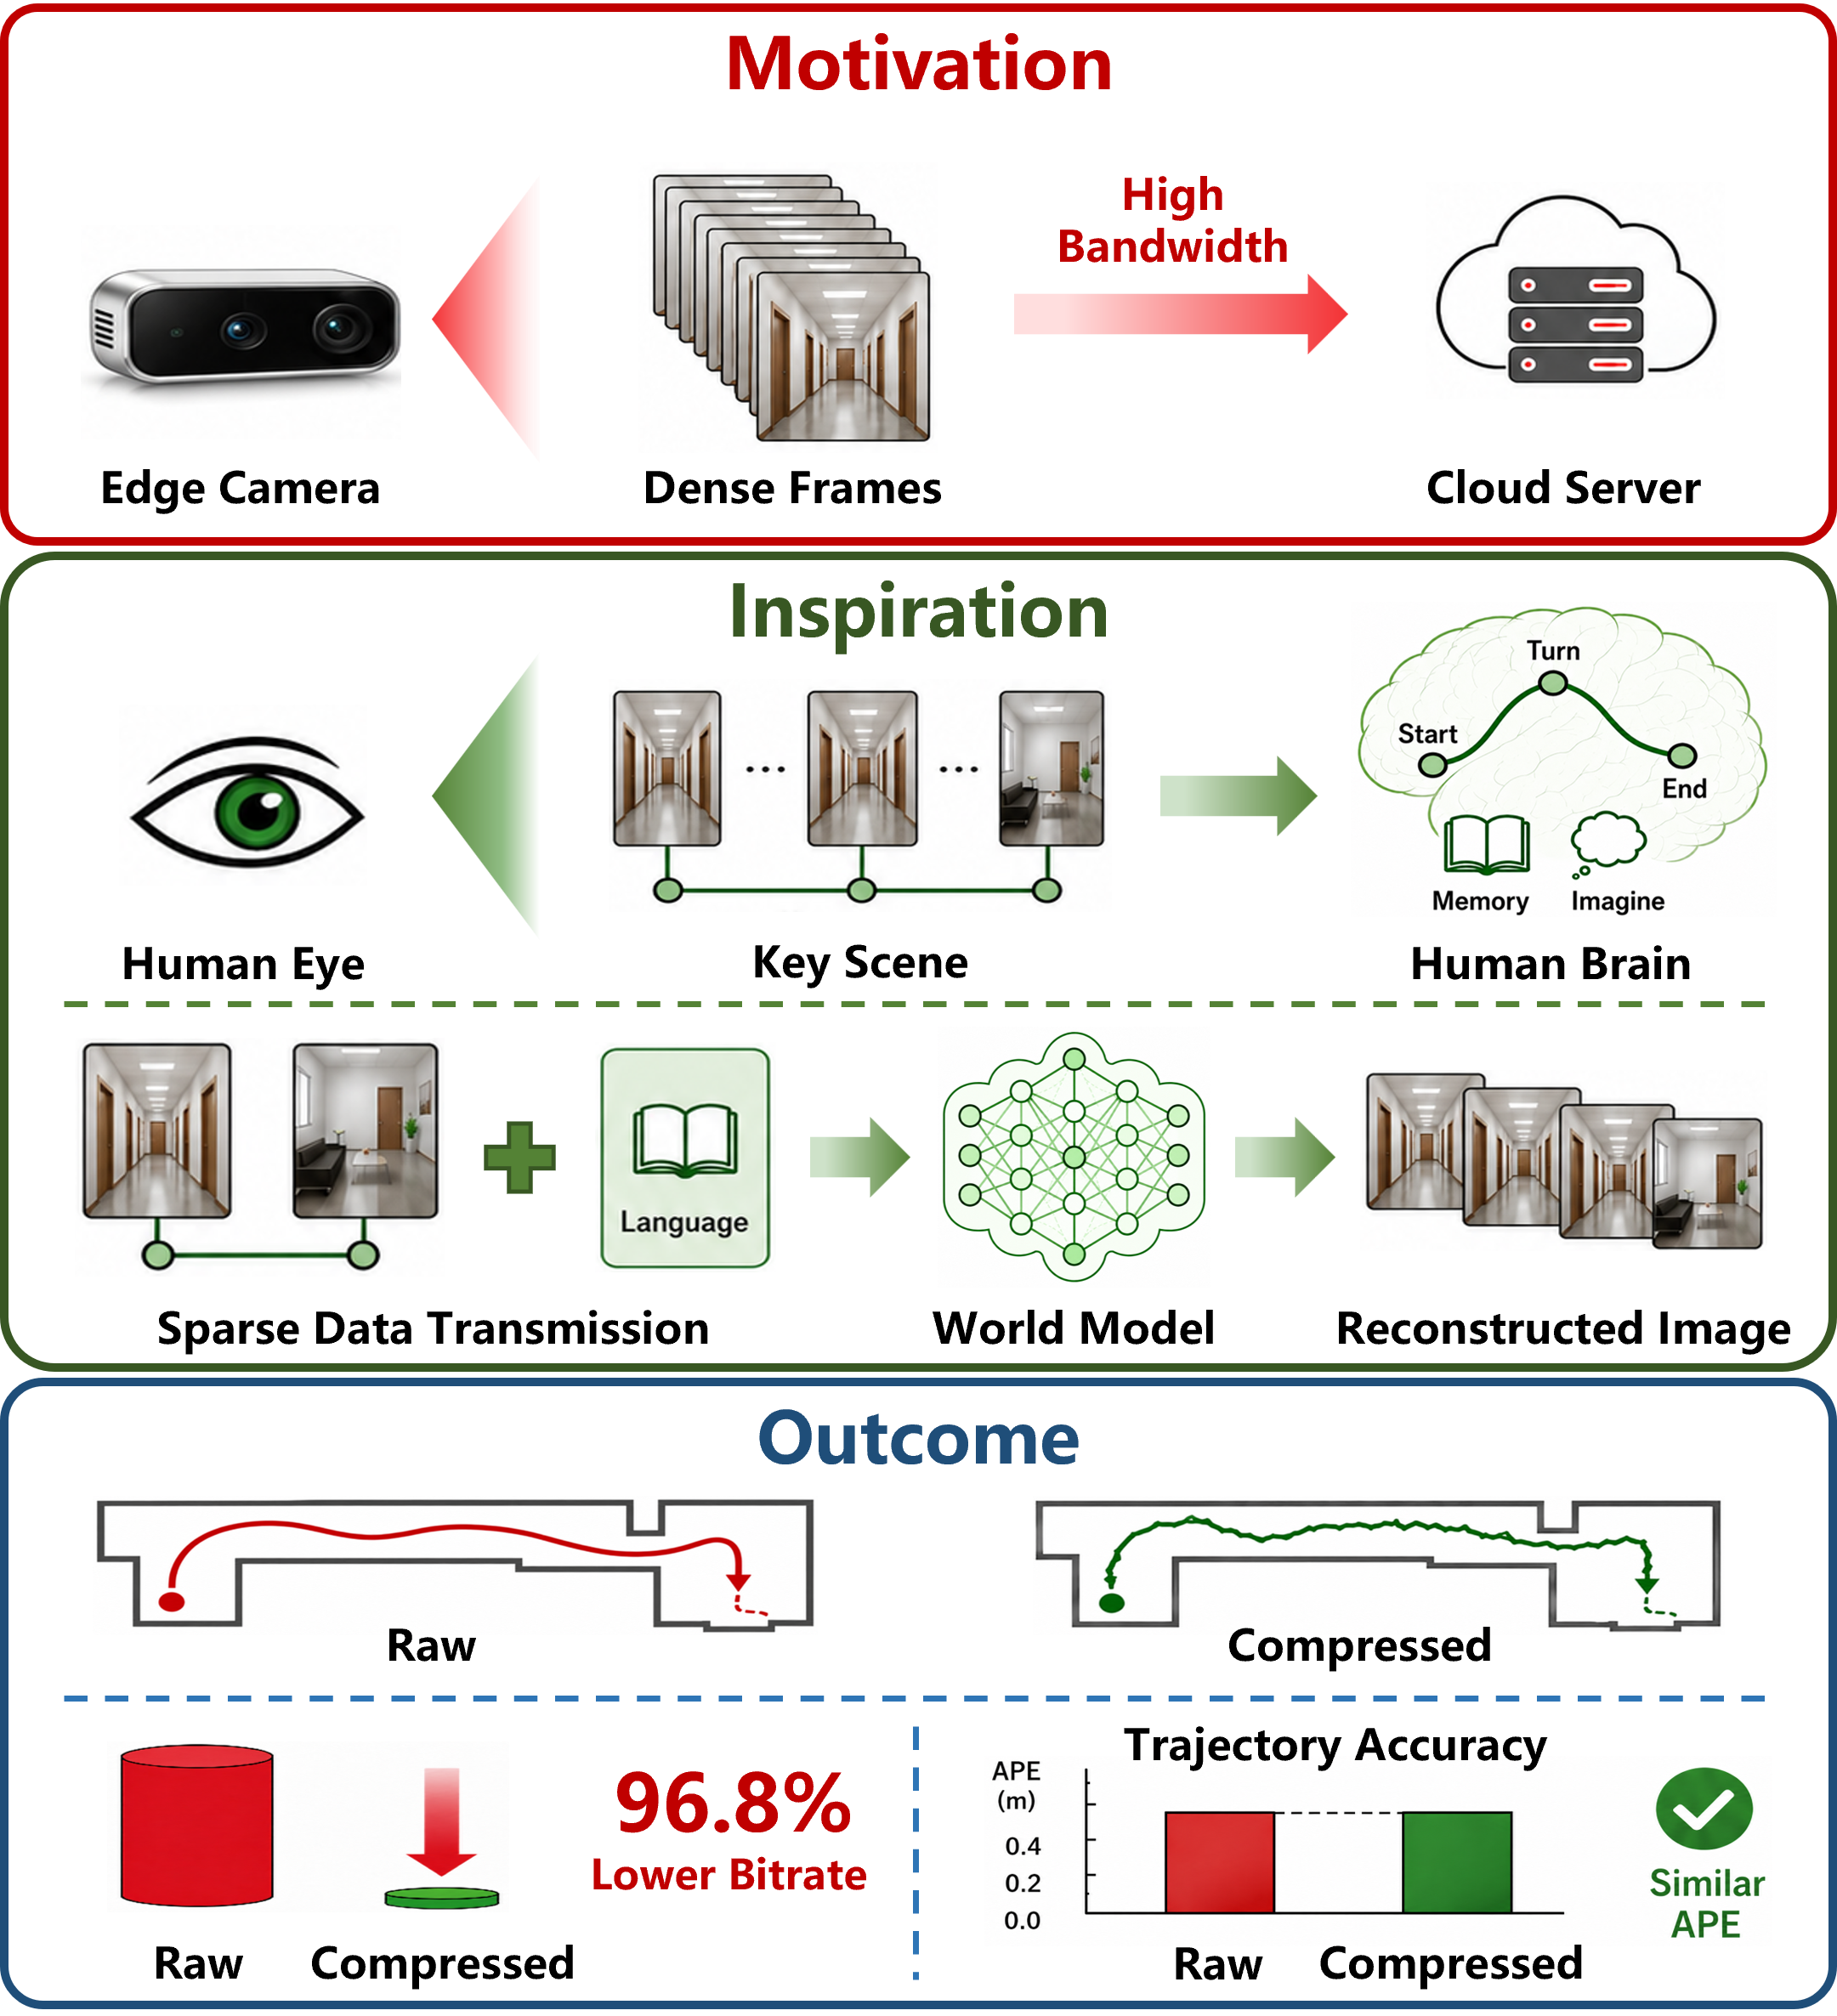
\includegraphics[width=0.95\columnwidth]{figures/fig1.png}
\caption{Motivation of human-inspired visual memory coding for edge--cloud VSLAM. Dense visual transmission requires high bandwidth, whereas the proposed memory-based formulation transmits sparse visual novelty anchors and compact language memory for task-oriented reconstruction.}
\label{fig:concept}
\end{figure}

Existing image and video compression standards reduce this burden by exploiting spatial and temporal pixel redundancy. Although such codecs are highly effective for human viewing, their rate--distortion objectives are not directly aligned with VSLAM. For VSLAM, utility depends less on pixel-identical reconstruction than on feature repeatability, geometric continuity, trackable visual textures, and temporally consistent camera motion. Under aggressive compression, images that remain visually acceptable to humans may lose stable local features, introduce temporal artifacts, or distort geometric cues used by downstream pose estimation. Therefore, edge--cloud VSLAM transmission should not be treated merely as conventional video delivery, but as a task-oriented visual transmission problem in which the transmitted representation is formulated and evaluated by downstream VSLAM utility. Fig.~\ref{fig:concept} conceptually illustrates this motivation, while the quantitative compression and trajectory tradeoffs are reported in Section~\ref{sec:experiments}.

As a design analogy, this paper is motivated by a human-inspired view of visual memory. When navigating through an environment, humans need not retain every pixel of every frame; they often recall sparse key scenes, landmarks, motion transitions, and high-level semantic impressions. This analogy does not provide a biological model, but it suggests an engineering representation for edge--cloud VSLAM image transmission: a dense visual stream can be represented by sparse image--text visual memories. In this representation, boundary frames provide geometric anchors, motion transitions and visual novelty anchors indicate what should be retained, language memory provides compact high-level conditions, and a cloud-side generative model reconstructs task-usable visual continuity.

Based on this formulation, we propose \emph{HVM-Codec}, a human-inspired image--text visual memory coding framework for edge--cloud VSLAM. For each visual memory unit, the edge transmits boundary frames as geometric constraints and constructs compact language memory to describe motion intent, scene priors, and reconstruction constraints. The boundary frames constrain the start and end appearance of the segment, while the language memory represents part of the omitted visual information with a lower-bit abstraction. The cloud-side image--text conditioned world-model decoder uses its learned visual prior to reconstruct task-usable intermediate frames. The reconstructed sequence is then fed into a cloud-side VSLAM backend for trajectory estimation.

The key mechanism behind HVM-Codec is the combination of three complementary information sources. First, boundary frames preserve visual and geometric constraints that are difficult to describe purely by language. Second, language memory encodes high-level motion and semantic priors with low communication cost. Third, the cloud-side world-model decoder supplies plausible intermediate visual continuity from its learned prior under the image--text constraints. In this way, dense visual transmission is reformulated as a compact image--text memory transmission problem rather than a generic video compression problem.

To make this framework practical for edge--cloud VSLAM, HVM-Codec adopts a lightweight edge-side memory encoder. Instead of running heavy online captioning or dense optical-flow networks on the edge, the encoder uses low-cost visual measurements to estimate coarse motion memory and visual novelty anchors. These cues are then converted into structured language memory through a controllable prompt vocabulary and motion-conditioned templates. In the cloud decoding stage, Low-Rank Adaptation (LoRA) produces a LoRA-tuned decoder that is biased toward navigation-style visual transitions and VSLAM-oriented reconstruction. In this work, reconstruction is evaluated primarily by downstream VSLAM trajectory accuracy using absolute pose error (APE) RMSE, while transmission reduction, edge-side motion-estimation cost, and auxiliary image-fidelity metrics are reported to characterize the tradeoffs.

The main contributions of this paper are summarized as follows:
\begin{itemize}
    \item We propose a human-inspired image--text visual memory coding framework for edge--cloud VSLAM that replaces dense frame transmission with sparse boundary frames and compact language memory.
    \item We design a lightweight edge-side visual memory encoder that selects boundary frames, extracts coarse motion memory and visual novelty cues, and converts them into compact language memory without relying on heavy online generative captioning.
    \item We develop an image--text conditioned cloud-side world-model decoder with LoRA adaptation for VSLAM-oriented reconstruction, where boundary frames and language memory jointly constrain task-usable intermediate-frame generation.
    \item We evaluate task-level edge--cloud visual transmission tradeoffs through compression and APE RMSE results, edge-side motion-estimation cost, and Base/LoRA decoder behavior with auxiliary LPIPS, SSIM, and FID metrics.
\end{itemize}

The remainder of this paper is organized as follows. Section~\ref{sec:related_work} reviews related work on edge--cloud VSLAM transmission, sparse visual memory coding for navigation, and world models for visual sequence reconstruction. Section~\ref{sec:methodology} presents the proposed HVM-Codec framework. Section~\ref{sec:experiments} reports the experimental evaluation and ablation studies. Section~\ref{sec:discussion} presents the discussion and limitations. Section~\ref{sec:conclusion} concludes the paper.

% !TEX root = ../main.tex

\section{Related Work}
\label{sec:related_work}
% ==================================================


\subsection{Edge--Cloud VSLAM Transmission}
\label{subsec:edge_cloud_transmission}

Visual SLAM has evolved from feature-based and direct pipelines to learning-based systems with stronger robustness. ORB-SLAM2 and ORB-SLAM3 build sparse maps from repeatable local features and optimize camera poses through bundle adjustment~\cite{murartal2017orbslam2,campos2021orbslam3}. Direct and semi-direct systems such as LSD-SLAM, DSO, and SVO exploit photometric consistency~\cite{engel2014lsdslam,engel2018dso,forster2014svo}, while learning-based systems such as DROID-SLAM introduce dense recurrent optimization across monocular, stereo, and RGB-D inputs~\cite{teed2021droidslam}. These advances improve localization and mapping capability, but they also increase computation and memory demand, motivating edge--cloud VSLAM for resource-constrained robots.

Early collaborative SLAM and cloud robotics systems move expensive mapping, optimization, or reconstruction modules from the robot to external computation resources~\cite{rabaud2011c2tam,kuffner2010cloud,shankar2020fogros}. Recent reviews identify transmission latency and data volume as central bottlenecks, and highlight asynchronous collaboration, submap allocation, and compact representation transmission as important directions~\cite{chen2024reviewcloudedge}. Submap-based edge--cloud VSLAM reduces transmission frequency by offloading selected image segments or submap construction to the cloud~\cite{chen2024cloudlearning,chen2024implicittransmission}. Implicit-representation transmission and VC-SLAM further reduce transferred map data by sending compact neural representations instead of dense point clouds or meshes~\cite{chen2024implicittransmission,huo2025vcslam}, while cross-representation methods study data association and adaptive representation selection for VSLAM~\cite{chen2024crossdata,chen2025xrepslam}.

These works show that edge--cloud VSLAM must reduce communication demand, but they mainly address task allocation, submap transmission, map representation, or data association after visual observations have already been selected. Conventional codecs such as H.264/AVC, H.265/HEVC, and H.266/VVC reduce image streams with rate--distortion objectives designed mainly for human viewing~\cite{sullivan2012h264,sullivan2012hevc,bross2021vvc}. Learned and generative compression exploit neural priors under limited bit budgets~\cite{balle2018variational,minnen2018joint,agustsson2020scale,mentzer2020highfidelity}, and semantic communication emphasizes transmitting task-relevant meaning rather than raw symbols~\cite{qin2021semantic,luo2022semantic}. HVM-Codec addresses the preceding VSLAM-oriented visual transmission problem: encoding the edge image stream itself as sparse image--text visual memory before cloud-side VSLAM, and evaluating that representation by downstream VSLAM trajectory quality.

\subsection{Sparse Visual Memory Coding for Navigation}
\label{subsec:sparse_visual_memory}

Sparse visual memory provides an engineering analogy for replacing dense frame transmission with compact navigation cues. Cognitive studies on event perception suggest that continuous experience can be segmented into events, with boundaries related to changes in prediction, attention, and memory~\cite{zacks2001event,zacks2007event}. Mental-model theory also emphasizes simplified internal representations that preserve structural relationships rather than exhaustive sensory details~\cite{johnsonlaird1983mental}. For VSLAM-oriented visual transmission, this analogy motivates retaining boundary frames, motion transitions, visual novelty anchors, and compact language memory instead of every intermediate frame.

Computer vision has studied related mechanisms through temporal segmentation, change-point detection, and event boundary detection. Generic Event Boundary Detection detects taxonomy-free boundaries according to human-perceived event changes~\cite{shou2021gebd}. Online Bayesian change-point detection provides a statistical foundation for streaming segmentation~\cite{adams2007bayesian}, and streaming representation learning organizes visual inputs into event-level structures~\cite{streamer2023}. Vision-language models such as CLIP and BLIP-2 connect visual content with compact language-level semantics~\cite{radford2021clip,li2023blip2}. In VSLAM, X-RepSLAM uses VLM-derived image-sequence information to guide adaptive representation switching and prompt-driven task customization~\cite{chen2025xrepslam}.

These works provide useful ingredients for segmentation and semantic representation, but they are not designed as a transmissible memory format for edge--cloud VSLAM. Event segmentation typically aims at video understanding or retrieval, and vision-language representations usually describe or select visual content rather than encode a sequence for later task-usable reconstruction. HVM-Codec uses motion memory and visual novelty anchors not only to segment the stream, but also to form image--text visual memory whose boundary frames and language memory are decoded and evaluated by downstream VSLAM.

\subsection{World Models for Visual Sequence Reconstruction}
\label{subsec:world_model_decoding}

World models provide learned priors for predicting or imagining visual continuity from sparse conditions. Ha and Schmidhuber revived the term ``world model'' by learning latent environment dynamics for agents that can simulate possible futures~\cite{ha2018worldmodels}. The Dreamer family demonstrates that latent world models can support decision-making and control through imagined rollouts~\cite{hafner2019planet,hafner2020dreamer,hafner2023dreamerv3}. JEPA-style predictive representation learning emphasizes predicting abstract latent representations rather than raw pixels~\cite{lecun2022path,assran2024vjepa}, and recent surveys categorize world models by their roles in constructing internal representations and predicting future states~\cite{ding2025worldmodelsurvey}.

Large-scale video generation is one visual realization of world models. Image-to-video and text-to-video diffusion models synthesize temporally coherent sequences from sparse visual or language conditions~\cite{blattmann2023svd,ho2022videodiffusion,villegas2022phenaki}. Sora, Genie, Cosmos, and related systems indicate that large video models can capture aspects of spatiotemporal consistency, controllability, and visual imagination, while still having limitations as physical simulators~\cite{brooks2024sora,bruce2024genie,nvidia2025cosmos}. In robotics and embodied AI, world models have been explored for learning from imagined futures, generating robot action videos, and supporting planning~\cite{yang2023unipi,du2023learning,wu2023daydreamer}. Target-Bench is especially relevant because it evaluates generated future videos for mapless path planning and compares recovered camera motion with SLAM-based ground truth trajectories~\cite{wang2025targetbench}.

Generic world models and video generators mainly emphasize future prediction, visual plausibility, realism, diversity, prompt adherence, or planning. VSLAM-oriented reconstruction instead requires stable viewpoints, geometric continuity, and trackable visual textures. Efficient low-rank adaptation such as LoRA makes it possible to bias a pretrained decoder toward a target domain without retraining the full model~\cite{hu2022lora}. HVM-Codec therefore treats the cloud module as an image--text conditioned world-model decoder constrained by sparse visual memory. Its output is not expected to be pixel-identical to the original stream; it is evaluated by task-usable reconstruction and downstream VSLAM trajectory quality.

% !TEX root = ../main.tex

% Local fallback because the template does not define \mathscr.
\providecommand{\mathscr}[1]{\mathcal{#1}}

% ==================================================

\section{Methodology}
\label{sec:methodology}
% ==================================================

\subsection{Framework Overview and Problem Formulation}
\label{subsec:framework_formulation}

\HVM{} formulates edge--cloud VSLAM transmission as a VSLAM-oriented vision--language memory coding problem. Instead of sending a dense image stream to the cloud, the edge device selects sparse boundary frames and summarizes the omitted intervals with motion memory, semantic anchors, and language memory. The cloud then reconstructs task-usable intermediate views with a vision--language conditioned world-model decoder, and the resulting visual stream is consumed by a conventional cloud-side VSLAM estimator.

\begin{figure*}[!t]
\centering
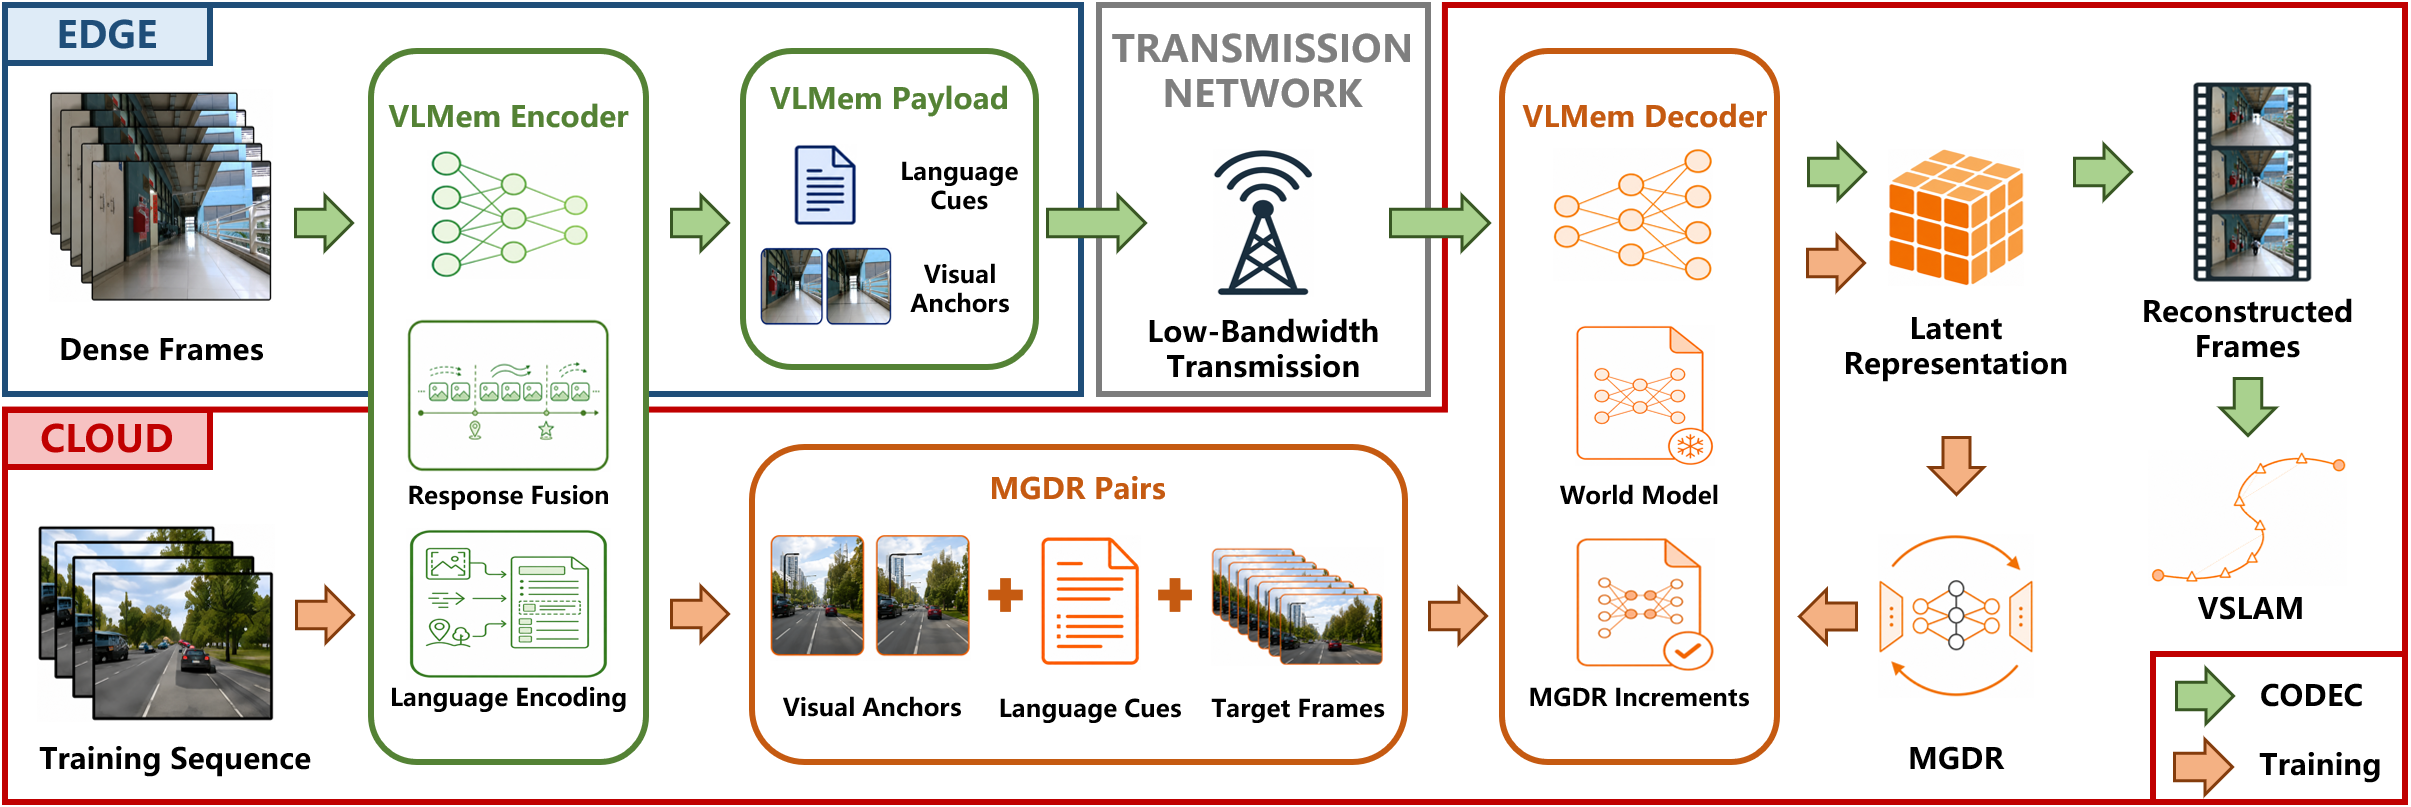
\includegraphics[width=\textwidth]{figures/fig2.png}
\caption{Overall framework of HVM-Codec for edge--cloud VSLAM visual transmission. The edge-side encoder converts dense visual streams into boundary frames, motion memory, semantic anchors, and compact language memory, while the cloud-side world-model decoder reconstructs task-usable visual sequences for downstream VSLAM. The same memory format is used for inference and memory-guided refinement.}
\label{fig:framework}
\end{figure*}

Fig.~\ref{fig:framework} gives the global pipeline. The edge device performs lightweight memory encoding over a fixed set of admissible temporal positions, transmits sparse vision--language memory, and leaves dense visual reconstruction to the cloud. The same memory format is used offline to prepare memory-guided refinement pairs, so the decoder observes consistent boundary-frame and language-memory conditions during refinement and inference.

Let the dense visual stream captured by the edge device be
\begin{equation}
\mathcal{I}_{1:T}
=\{I_t\}_{t=1}^{T},\qquad
I_t\in\mathbb{R}^{H\times W\times C}.
\label{eq:dense_stream}
\end{equation}
Here \(I_t\) is the \(t\)-th image in a sequence of length \(T\), and \(H\), \(W\), and \(C\) denote image height, width, and channels.

The edge encoder represents omitted intervals by vision--language memory units. Let \(\mathcal{P}\subseteq\{1,\ldots,T\}\) denote the admissible temporal positions from which boundaries and anchor candidates may be selected. Unit \(i\) is
\begin{equation}
\begin{aligned}
\mathcal{U}_i
=\big(&I_{b_i^-},I_{b_i^+},\mathcal{S}_i,\mathcal{A}_i,\\
&\mathcal{L}_i,\mathcal{L}_i^{-}\big),\qquad
b_i^-,b_i^+\in\mathcal{P}.
\end{aligned}
\label{eq:vl_memory_unit}
\end{equation}
The boundary frames \(I_{b_i^-}\) and \(I_{b_i^+}\) provide geometric and appearance constraints at the ends of the unit. The variable \(\mathcal{S}_i\) is motion memory, \(\mathcal{A}_i\) is the set of semantic anchors, and \(\mathcal{L}_i\) and \(\mathcal{L}_i^{-}\) are positive and negative language memory.

The edge-side memory encoder \(\mathcal{E}_{\phi}\) and cloud-side world-model decoder \(\mathcal{G}_{\theta+\Delta\theta}\) are written compactly as
\begin{equation}
\begin{aligned}
\mathcal{M}
&=\mathcal{E}_{\phi}(\mathcal{I}_{1:T};\mathcal{P})
=\{\mathcal{U}_i\}_{i=1}^{N},\\
\widehat{\mathcal{I}}_{1:T}
&=\mathcal{G}_{\theta+\Delta\theta}(\mathcal{M}).
\end{aligned}
\label{eq:memory_coding}
\end{equation}
The memory \(\mathcal{M}\) is not a conventional pixel bitstream. It is sparse vision--language memory containing boundary frames, motion memory, semantic-anchor indicators, language memory, and metadata needed for task-usable visual reconstruction on the cloud side. The increment \(\Delta\theta\) denotes optional decoder refinement increments applied to the pretrained decoder; Sec.~\ref{subsec:wm_lora_decoding} instantiates these increments with LoRA. With \(\Delta\theta=0\), the same notation describes the original unrefined world-model decoder. The small constant \(\epsilon\) used in later normalized ratios is introduced only for stable normalization.

Let \(\mathcal{B}\) denote the boundary positions and let \(\mathcal{K}=\{I_b\mid b\in\mathcal{B}\}\) be the transmitted boundary-frame set. The transmission cost is
\begin{equation}
\begin{aligned}
\mathcal{R}(\mathcal{M})
=&\mathcal{R}(\mathcal{K})
+\sum_{i=1}^{N}
\mathcal{R}(\mathcal{S}_i,\mathcal{A}_i,\mathcal{L}_i,\mathcal{L}_i^{-})\\
&+\mathcal{R}(\mathrm{meta}),\qquad
\mathcal{K}=\{I_b\mid b\in\mathcal{B}\}.
\end{aligned}
\label{eq:transmission_cost}
\end{equation}
Here \(\mathcal{R}(\cdot)\) denotes payload size. The compact memory term covers motion memory, semantic-anchor indicators, and language memory; Eq.~\eqref{eq:transmission_cost} is a rate model for reasoning about payload, not a claim that all components contribute equally.

The VSLAM-oriented rate--trajectory design criterion is
\begin{equation}
\begin{aligned}
\mathcal{M}^{\star}
=\arg\min_{\mathcal{M}\in\Omega}\;
&\mathcal{R}(\mathcal{M})\\
&+\lambda\mathcal{D}_{\mathrm{slam}}\!\left(
\mathcal{F}_{\mathrm{slam}}(\widehat{\mathcal{I}}_{1:T}),
\mathcal{T}\right).
\end{aligned}
\label{eq:rate_trajectory_design}
\end{equation}
Here \(\Omega\) is the admissible family of memory representations, \(\lambda\) is the trade-off coefficient between transmission cost and downstream trajectory discrepancy, \(\mathcal{F}_{\mathrm{slam}}\) is the cloud-side VSLAM estimator, \(\mathcal{T}\) is the reference trajectory when available, and \(\mathcal{D}_{\mathrm{slam}}\) is evaluated through APE RMSE in the experiments.

Eq.~\eqref{eq:rate_trajectory_design} is a VSLAM-oriented rate--trajectory design criterion rather than a closed-form optimization solved by the implementation. Conventional rate--distortion coding usually measures pixel distortion or perceptual reconstruction error. HVM-Codec instead treats task distortion as downstream VSLAM trajectory quality after task-usable visual reconstruction. In this paper, the two sides of the criterion are evaluated empirically through payload size and APE RMSE, while auxiliary image-fidelity metrics are reported separately.

\subsection{Motion--Semantic Event Memory Encoding}
\label{subsec:motion_semantic_segmentation}

The edge encoder constructs memory units from two complementary cues: a block-wise motion trend response and a semantic-anchor response. The motion trend response identifies forward motion, turning, and mixed transitions that affect viewpoint continuity. Semantic anchors capture embedding-level scene/content changes that should constrain admissible unit spans even when the coarse motion regime remains stable.

\begin{figure*}[!t]
\centering
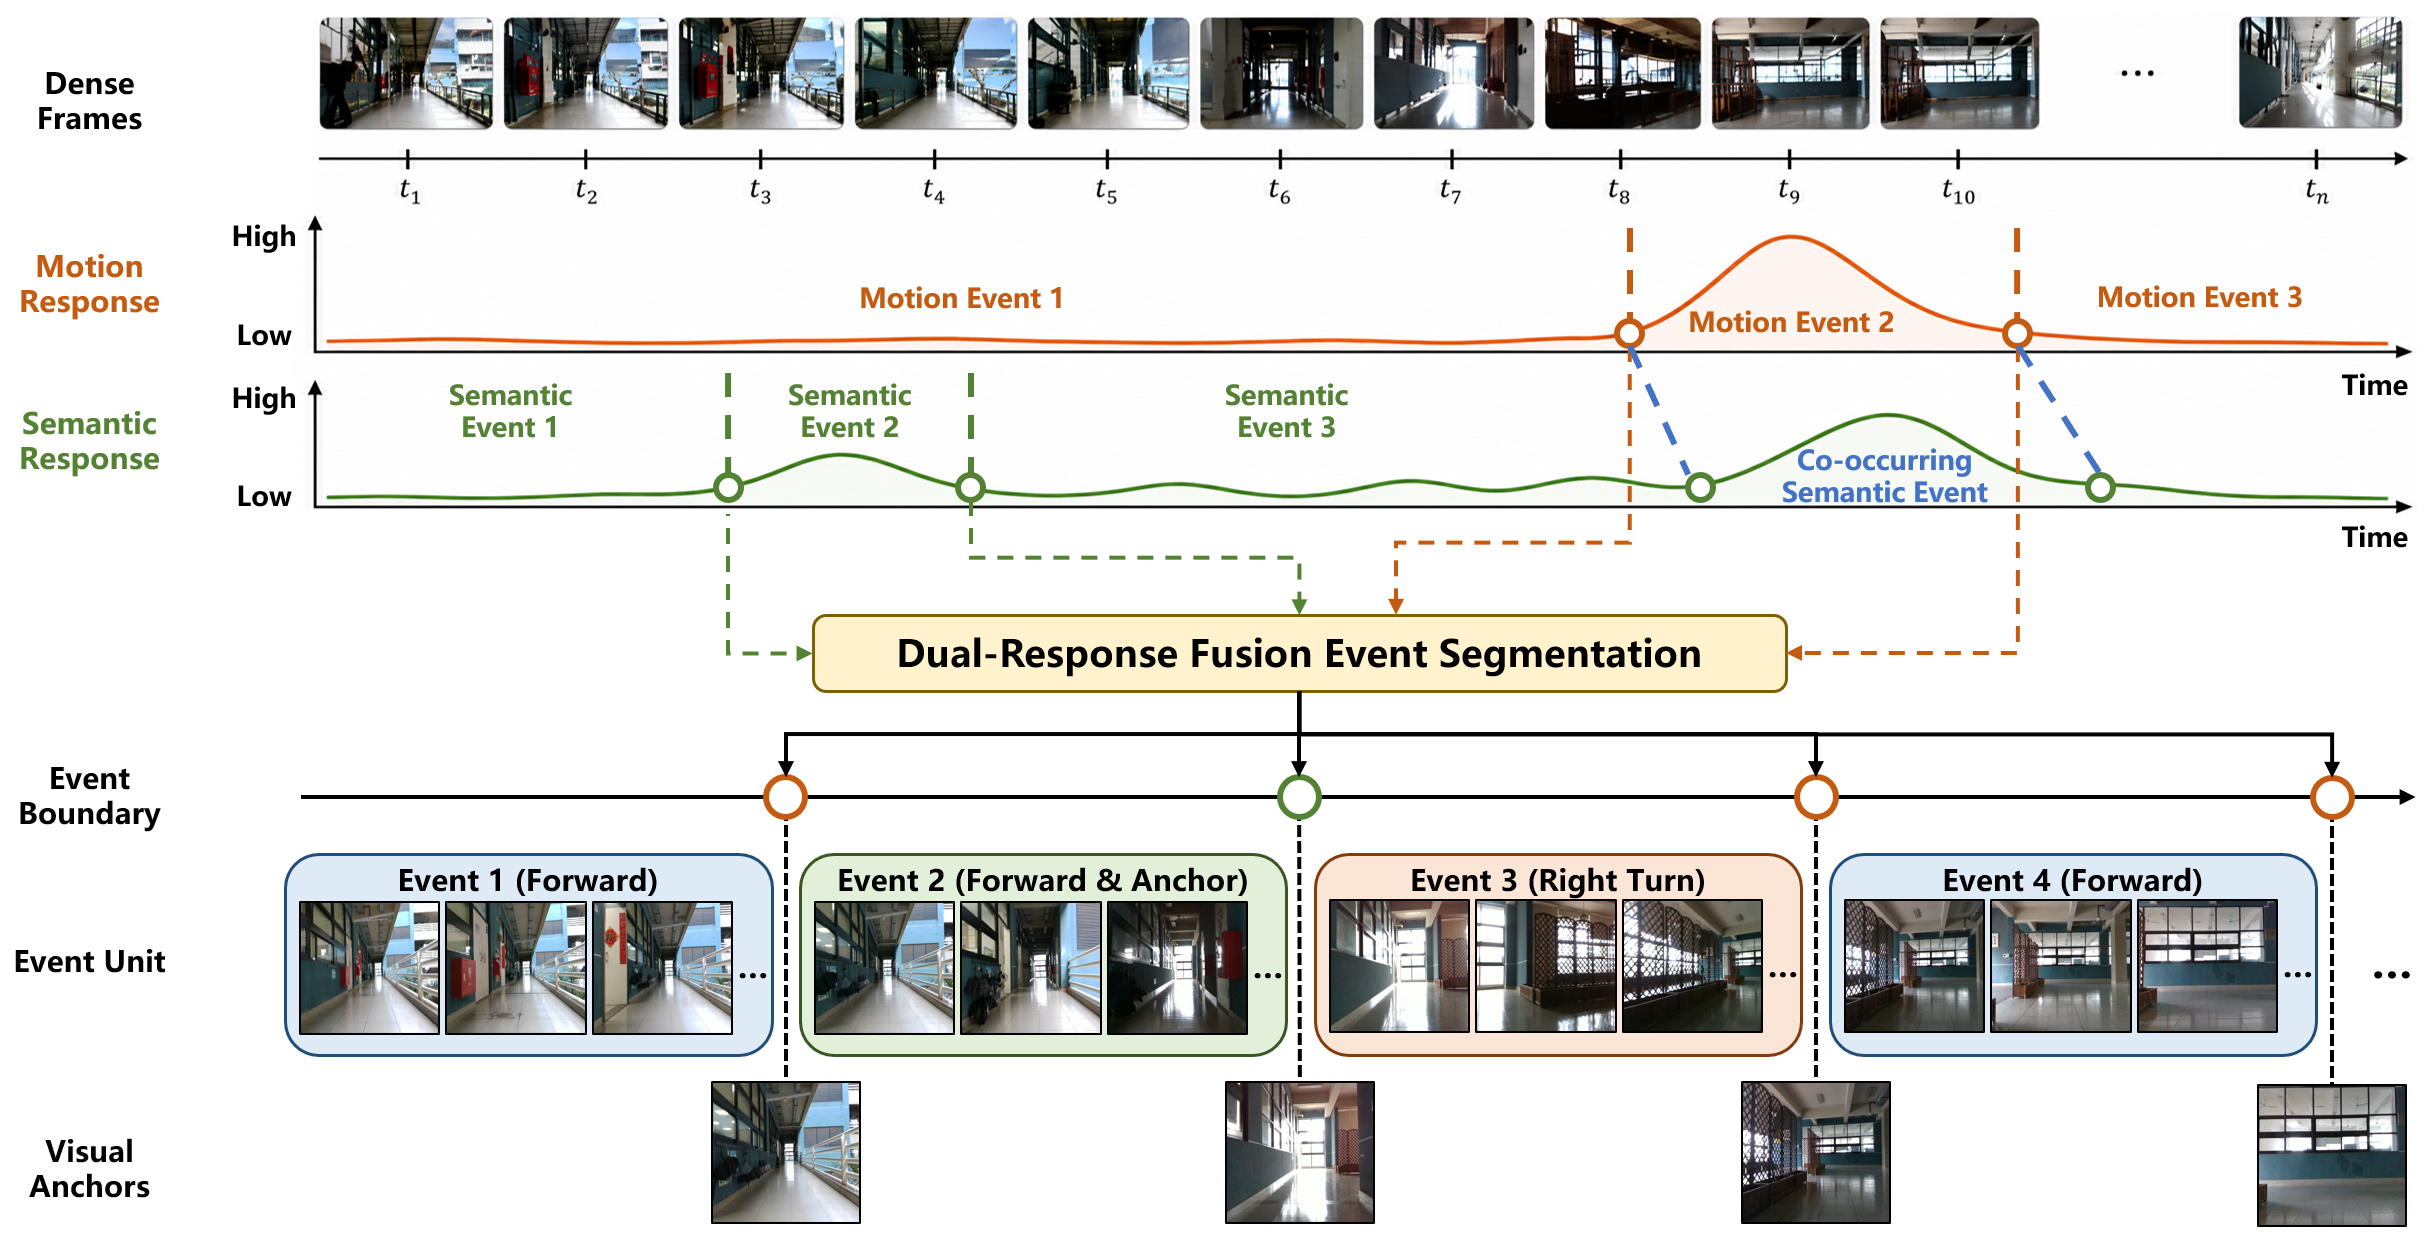
\includegraphics[width=0.92\textwidth]{figures/fig3.png}
\caption{Motion--semantic response fusion. Motion trend responses and semantic anchor responses are fused to divide the dense visual stream into vision--language memory units. Each unit is represented by boundary frames, motion memory, semantic anchors, and compact language memory.}
\label{fig:event_segmentation}
\end{figure*}

As shown in Fig.~\ref{fig:event_segmentation}, the encoder estimates low-cost motion trend response between consecutive frames by block-wise phase correlation. The encoder does not require dense pixel-level correspondence; it needs motion-regime-level evidence for boundary construction and motion-conditioned language memory. Each frame is divided into spatial blocks indexed by \(g\), \(I_t^g\) denotes the corresponding image patch, and \(H\) is a local windowing mask. The phase-correlation response is
\begin{equation}
\begin{aligned}
\widetilde{I}_{t}^{g}
&=H\odot I_t^g,\\
\mathcal{C}_{t,g}
&=\mathscr{F}^{-1}\!\left(
\frac{
\mathscr{F}(\widetilde{I}_{t}^{g})
\mathscr{F}(\widetilde{I}_{t-1}^{g})^{*}}
{\left|
\mathscr{F}(\widetilde{I}_{t}^{g})
\mathscr{F}(\widetilde{I}_{t-1}^{g})^{*}
\right|+\epsilon}\right),\\
(\mathbf{d}_{t,g},\rho_{t,g})
&=\operatorname{Peak}(\mathcal{C}_{t,g}).
\end{aligned}
\label{eq:block_phase_correlation}
\end{equation}
Here \(\odot\) denotes element-wise multiplication, \(\mathscr{F}\) is the Fourier transform, \((\cdot)^{*}\) is complex conjugation, \(\mathbf{d}_{t,g}\) is the block displacement, and \(\rho_{t,g}\) is the peak confidence. The block-wise form provides a lightweight trend cue without dense optical flow. Because each block contributes a local displacement peak, the following aggregation can capture coarse camera behavior while staying inexpensive enough for edge-side memory encoding.

The encoder downweights blocks whose phase-correlation peaks or visual texture are unreliable. This is summarized by the reliability function
\begin{equation}
w_{t,g}
=\omega_{\mathrm{rel}}
\left(
\rho_{t,g},
\sigma(I_{t-1}^{g}),
g
\right).
\label{eq:block_reliability}
\end{equation}
The function \(\omega_{\mathrm{rel}}\) combines peak confidence, local texture strength \(\sigma(I_{t-1}^{g})\), and row-position reliability. It suppresses weakly textured or unreliable blocks before the motion descriptors are accumulated. This reliability weighting is important because texture-poor regions and unstable block peaks can otherwise dominate a simple average and create spurious motion-regime changes.

The weighted block displacements define two compact motion descriptors:
\begin{equation}
\begin{aligned}
\bar{\mathbf{d}}_{t}
&=
\frac{\sum_g w_{t,g}\mathbf{d}_{t,g}}
{\sum_g w_{t,g}+\epsilon},\\
\chi_t
&=
\frac{\sum_g w_{t,g}
\left(x'_g d^{x}_{t,g}+y'_g d^{y}_{t,g}\right)}
{\sum_g w_{t,g}\left((x'_g)^2+(y'_g)^2\right)+\epsilon}.
\end{aligned}
\label{eq:motion_descriptors}
\end{equation}
Here \(\bar{\mathbf{d}}_t\) is the reliability-weighted global displacement trend, \(\chi_t\) is radial expansion evidence related to forward motion, and \((x'_g,y'_g)\) are normalized block-center coordinates.

The descriptors are converted into motion trend scores and a coarse motion regime. Let \(\zeta_t\) denote the yaw-like lateral response derived from the reliability-weighted block displacement field:
\begin{equation}
\begin{aligned}
r_t^{\mathrm{turn}}
&=\frac{|\zeta_t|}{s_m+\epsilon}c_t^{\mathrm{sgn}},
\qquad
r_t^{\mathrm{fwd}}
=\frac{\max(\chi_t,0)}{s_m+\epsilon}c_t^{\mathrm{exp}},\\
s_t
&=\Gamma_m(r_t^{\mathrm{turn}},
r_t^{\mathrm{fwd}},c_t^{\mathrm{sgn}}),
\qquad
s_t\in\mathcal{S}_{\mathrm{motion}}.
\end{aligned}
\label{eq:motion_regime_assignment}
\end{equation}
The scalar \(s_m\) normalizes the motion scale, \(c_t^{\mathrm{sgn}}\) measures left/right sign consistency, and \(c_t^{\mathrm{exp}}\) measures expansion consistency. The rule \(\Gamma_m\) is a lightweight mapping from motion trend scores to coarse motion regimes such as forward, left-turn, right-turn, and mixed; it is not a learned classifier.

Frame-level regimes are stabilized over admissible temporal windows:
\begin{equation}
\begin{aligned}
\ell_j
&=\Gamma_w(\{s_t,r_t^{\mathrm{turn}},
r_t^{\mathrm{fwd}},\rho_t\}_{t\in W_j}),\\
\widetilde{\ell}_j
&=\operatorname{Stab}_{\tau_\rho}
(\ell_{j-1},\ell_j,\ell_{j+1},\bar{\rho}_j).
\end{aligned}
\label{eq:window_stabilization}
\end{equation}
Here \(W_j\) is an admissible temporal window, \(\rho_t\) is frame-level confidence aggregated from block responses, and \(\bar{\rho}_j\) is the window-average confidence. The label \(\ell_j\) is the window-level motion regime, while \(\widetilde{\ell}_j\) suppresses isolated low-confidence regime changes when neighboring windows agree. This stabilization is needed because frame-level motion evidence can be noisy, especially near weak texture or transient viewpoint changes. By preserving persistent transitions while suppressing unreliable one-window changes, it reduces unnecessary fragmentation of the memory representation.

Semantic anchors complement motion memory by detecting embedding-level scene/content changes. For a candidate admissible position \(p\) and current semantic context \(c\), define
\begin{equation}
\begin{aligned}
\mathbf{z}_{p}
&=\frac{f_{\psi}(I_p)}{\|f_{\psi}(I_p)\|_2},
\qquad
r_p^{\mathrm{sem}}(c)=1-\mathbf{z}_{p}^{\top}\mathbf{z}_{c},\\
\mathcal{A}
&=\Big\{a\in\mathcal{P}\ \Big|
\operatorname{Pers}_{P_{\min}}
\big(r_a^{\mathrm{sem}}(c)>\tau_a(s)\big),\\
&\qquad\qquad
\operatorname{Sep}(a;c,b^+)\ge g_{\min}\Big\}.
\end{aligned}
\label{eq:semantic_anchor_admission}
\end{equation}
Here \(f_{\psi}\) is the image embedding encoder, \(\mathbf{z}_{p}\) and \(\mathbf{z}_{c}\) are normalized embeddings, and \(r_p^{\mathrm{sem}}(c)\) is the semantic-anchor response relative to the current semantic context \(c\). The context \(c\) need not be the immediately preceding frame; it represents the active scene/content reference used for the current interval. The operator \(\operatorname{Pers}_{P_{\min}}\) requires enough supporting admissible positions, and \(\operatorname{Sep}\) enforces separation from the semantic context and the unit boundary. The threshold \(\tau_a(s)\) depends on the motion regime \(s\), and \(\mathrm{turn}\) denotes either left-turn or right-turn regimes. Semantic anchors are embedding-level scene/content changes rather than hand-labeled object categories.

Finally, semantic anchors and admissible unit spans are combined through sequential boundary construction. Let \(\Delta_s\) be the motion-regime-dependent admissible unit span set and \(e\) the endpoint of the current interval:
\begin{equation}
\begin{aligned}
\mathcal{N}_k
&=\{p\in\mathcal{P}\mid b_k<p\le e,\;
p-b_k\in\Delta_s,\\
&\qquad\operatorname{Reach}(p,e;\Delta_s)=1\},\\
b_{k+1}
&=
\begin{cases}
\min(\mathcal{N}_k\cap\mathcal{A}),
& \mathcal{N}_k\cap\mathcal{A}\neq\varnothing,\\
\max\mathcal{N}_k, & \mathrm{otherwise}.
\end{cases}
\end{aligned}
\label{eq:admissible_boundary_construction}
\end{equation}
Here \(\mathcal{N}_k\) is the set of admissible next boundary positions from the current boundary \(b_k\), and \(\operatorname{Reach}(p,e;\Delta_s)\) ensures that the remaining interval can still be covered by valid spans. The construction chooses the earliest admissible semantic anchor when one is available; otherwise, it advances to the farthest reachable admissible boundary. This is a sequential construction, not a global optimization.

The complete event-memory encoding in III-B therefore has three stages. Block-wise phase correlation provides a low-cost motion trend response, semantic-anchor response adds embedding-level scene/content-change constraints, and admissible boundary construction combines both cues into vision--language memory units. The two responses are complementary: motion cues shorten difficult turn and mixed intervals where viewpoint change is harder to reconstruct, while semantic anchors prevent long stable-motion intervals from becoming visually underconstrained.

\subsection{Dual-Branch World-Model Decoding}
\label{subsec:wm_lora_decoding}

The cloud-side decoder has two coupled branches. The inference branch reconstructs task-usable intermediate frames from the transmitted vision--language memory, while the refinement branch performs \emph{memory-guided world-model refinement}. This refinement uses the same memory format as inference, exposing the decoder during refinement to the same type of boundary frames and language memory that it receives during deployment.

\begin{figure}[!t]
\centering
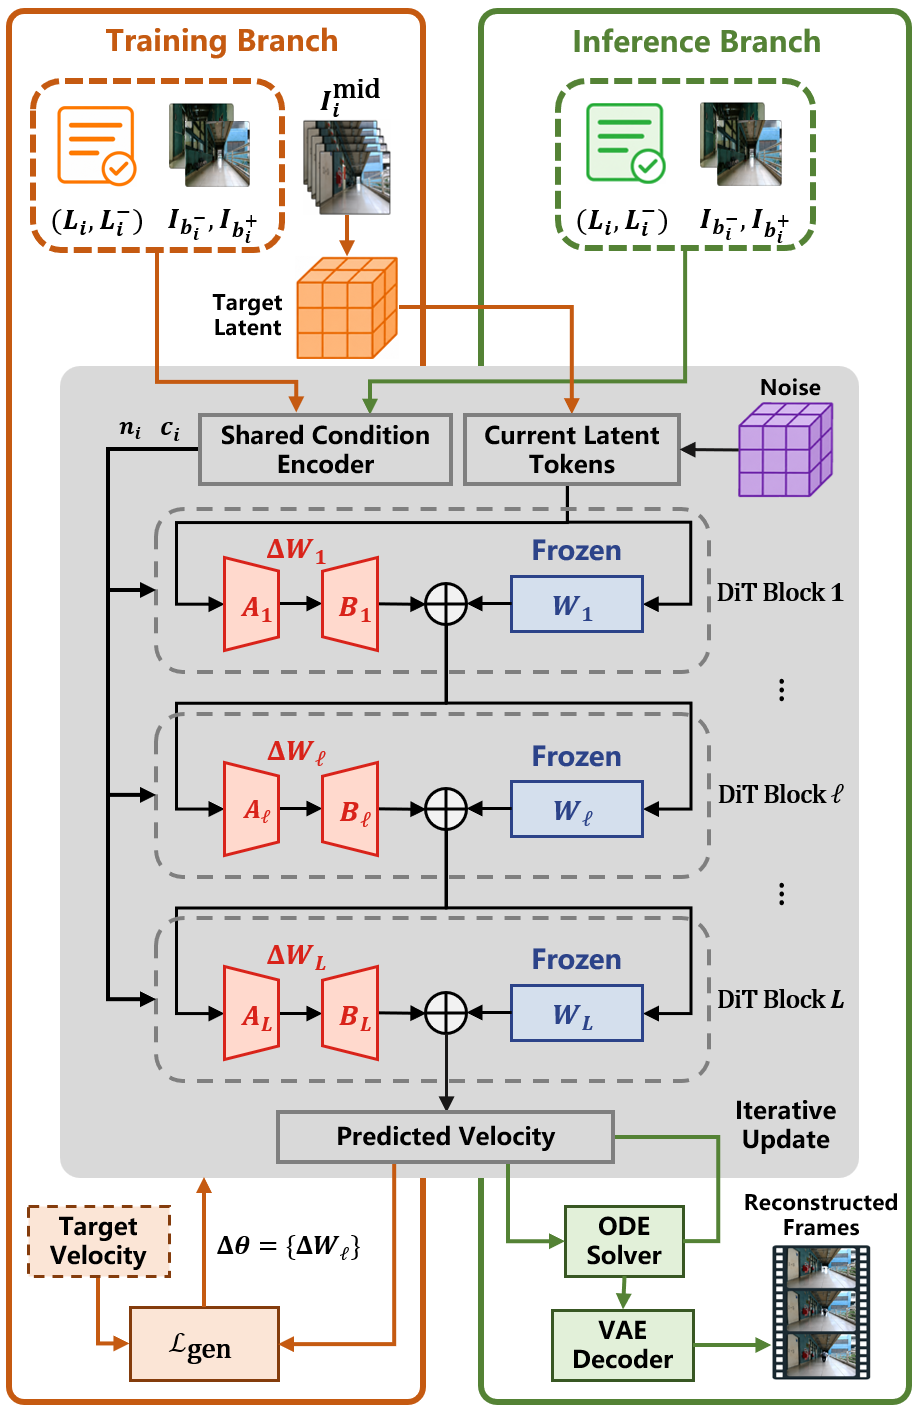
\includegraphics[width=0.95\columnwidth]{figures/fig4.png}
\caption{Dual-branch world-model decoding. The inference branch reconstructs intermediate frames from transmitted boundary frames and language memory. The refinement branch uses the same memory format to construct LoRA-based refinement pairs while keeping the pretrained world model frozen.}
\label{fig:lora_decoder}
\end{figure}

Fig.~\ref{fig:lora_decoder} illustrates the two branches. Boundary frames provide visual constraints that language memory cannot precisely express, while language memory supplies compact motion-conditioned priors for the omitted interval. First, each unit forms language memory from the shared navigation prior and the motion regime:
\begin{equation}
\begin{aligned}
\mathcal{L}_i
&=\operatorname{Join}\left(
\mathcal{L}_{\mathrm{base}},
\mathcal{L}_{\mathrm{motion}}(s_i)\right),\\
\mathcal{L}_i^{-}
&=\mathcal{L}_{\mathrm{neg}}.
\end{aligned}
\label{eq:language_memory_construction}
\end{equation}
The base term \(\mathcal{L}_{\mathrm{base}}\) provides the shared navigation-view prior, and \(\mathcal{L}_{\mathrm{motion}}(s_i)\) injects compact motion-conditioned language memory. The negative memory \(\mathcal{L}_{\mathrm{neg}}\) discourages blur, distortion, drift, sudden viewpoint jumps, and hallucinated objects. Semantic anchors influence unit boundaries and reconstruction intervals rather than being inserted as free-form text.

The decoder then reconstructs the omitted intermediate interval under boundary-frame and language-memory conditions:
\begin{equation}
\begin{aligned}
\widehat{\mathcal{I}}_{i}^{\mathrm{mid}}
&=
\mathcal{G}_{\theta+\Delta\theta}
\left(I_{b_i^-},I_{b_i^+},\mathcal{L}_i,\mathcal{L}_i^{-}\right),\\
b_i^+&=b_{i+1}^{-}.
\end{aligned}
\label{eq:conditional_reconstruction}
\end{equation}
The two boundary frames retain endpoint appearance and geometric cues, while language memory provides the coarse motion and reconstruction-quality prior for the interval. The shared-boundary condition \(b_i^+=b_{i+1}^{-}\) preserves continuity between neighboring units before the reconstructed sequence is passed to the VSLAM estimator. This is conditional world-model reconstruction, not conventional bitstream decoding.

For memory-guided refinement, raw training sequences are converted into pairs that use the same memory format as deployment:
\begin{equation}
\begin{aligned}
\mathcal{D}_{\mathrm{ref}}
&=\{(c_i,\mathcal{I}_{i}^{\mathrm{mid}})\}_{i=1}^{N_d},\\
c_i
&=\left(I_{b_i^-},I_{b_i^+},
\mathcal{L}_i,\mathcal{L}_i^{-}\right).
\end{aligned}
\label{eq:refinement_pairs}
\end{equation}
Here \(c_i\) is the conditioning tuple, and \(\mathcal{I}_{i}^{\mathrm{mid}}\) is the original intermediate-frame interval used as the target. These memory-guided refinement pairs use the same boundary-frame and language-memory format as inference, aligning refinement with deployment conditions and reducing the mismatch between refinement inputs and deployed memory units.

The implementation realizes memory-guided refinement with LoRA while keeping the pretrained world model frozen. For a selected layer weight \(W_{\ell}\), the low-rank increment is
\begin{equation}
\begin{aligned}
\Delta W_{\ell}
&=\frac{\alpha_{\ell}}{r}B_{\ell}A_{\ell},\qquad
A_{\ell}\in\mathbb{R}^{r\times d_{\ell}},\\
B_{\ell}&\in\mathbb{R}^{d'_{\ell}\times r},\qquad
r\ll\min(d_{\ell},d'_{\ell}).
\end{aligned}
\label{eq:lora_refinement_space}
\end{equation}
Here \(W_\ell\) is a selected layer weight, \(\Delta W_{\ell}\) is its low-rank increment, \(r\) is the low rank, \(\alpha_{\ell}\) is a layer scale, and only \(A_{\ell}\) and \(B_{\ell}\) are trainable while the pretrained world model remains frozen. Across selected layers, \(\Delta\theta\) denotes the collection of these low-rank increments \(\{\Delta W_\ell\}\). LoRA is therefore the lightweight implementation mechanism for memory-guided world-model refinement, not the core coding representation itself.

The refinement objective is defined over the memory-guided refinement pairs:
\begin{equation}
\begin{aligned}
\Delta\theta^{\star}
&=
\arg\min_{\Delta\theta\in\mathcal{H}_{\mathrm{LoRA}}}
\sum_{(c_i,\mathcal{I}_{i}^{\mathrm{mid}})\in\mathcal{D}_{\mathrm{ref}}}\\
&\qquad
\mathcal{L}_{\mathrm{gen}}\!\left(
\mathcal{G}_{\theta+\Delta\theta}(c_i),
\mathcal{I}_{i}^{\mathrm{mid}}\right).
\end{aligned}
\label{eq:memory_guided_refinement}
\end{equation}
Here \(\mathcal{H}_{\mathrm{LoRA}}\) is the space of LoRA-constrained parameter increments, and \(\mathcal{L}_{\mathrm{gen}}\) is the generation training loss of the underlying video world model. The objective exposes the decoder to the same memory-guided refinement pairs used to define the conditional reconstruction interface, so refinement follows the memory format rather than a separate supervision view.

The purpose of memory-guided refinement is to bias reconstruction toward navigation-style transitions, viewpoint stability, geometric continuity, and trackable structures under the same memory conditions used at inference. This bias does not imply artifact-free reconstruction or physical accuracy. The reconstructed frames remain task-usable visual reconstructions, and their value is assessed primarily through downstream VSLAM trajectory quality and the ablation study.

% !TEX root = ../main.tex

\section{Experimental Evaluation}
\label{sec:experiments}
% ==================================================

% Keep the project macro from swallowing spaces in this and following sections.
\makeatletter
\renewcommand{\HVM}{HVM-Codec\futurelet\@let@token\HVM@space}
\newcommand{\HVM@space}{%
  \ifx\@let@token\bgroup\else
  \ifx\@let@token,\else
  \ifx\@let@token.\else
  \ifx\@let@token;\else
  \ifx\@let@token:\else
  \ifx\@let@token)\else
  \ifx\@let@token]\else
  \space
  \fi\fi\fi\fi\fi\fi\fi}
\makeatother

\subsection{Experimental Setup}
\label{subsec:exp_setup}

The evaluation uses three types of sequences: NCD, TUM, and GDUT. NCD and TUM provide public benchmark sequences, while GDUT contains real robot data collected in our deployment environment. This combination allows the experiments to cover both standard datasets and robot-captured visual streams under the same \HVM{} evaluation protocol.

All experiments follow a unified prepare--encode--decode--eval pipeline. The preparation stage organizes image sequences and trajectory references; the encoder converts dense frames into the transmitted \HVM{} representation; the decoder produces a generated visual sequence from the image--text memory; and the evaluation stage runs the VSLAM backend on both original and generated sequences. Unless otherwise stated, phase correlation (PC) is used as the default lightweight motion estimator on the edge side. The cloud side uses an image--text conditioned world-model decoder, with Base and LoRA variants compared in the ablation study.

Trajectory quality is measured from the VSLAM backend output using evo after Sim(3) alignment, and the reported task metric is APE RMSE. Compression is measured by comparing the size of the original image sequence with the size of the transmitted \HVM{} representation. LPIPS, SSIM, and FID are used only as auxiliary image-fidelity metrics in the LoRA ablation; they are not the final task-level objective of \HVM.

\subsection{End-to-End Compression and VSLAM Accuracy}
\label{subsec:compression_accuracy}

The first experiment evaluates end-to-end transmission reduction and VSLAM trajectory accuracy across nine test fragments.

% This table is included by sections/04_experiments.tex.
\begin{table*}[!t]
\renewcommand{\arraystretch}{1.14}
\caption{End-to-end compression and VSLAM trajectory accuracy with GT path-length context.}
\label{tab:compression_accuracy}
\centering
\footnotesize
\setlength{\tabcolsep}{2pt}
\begin{tabular*}{\textwidth}{@{\extracolsep{\fill}}cc*{8}{c}@{}}
\toprule
\multirow{2}{*}{Dataset} & \multirow{2}{*}{Seq.} & \multirow{2}{*}{$L_{\mathrm{GT}}$ (m)} & \multicolumn{3}{c}{Payload} & \multicolumn{3}{c}{APE RMSE} & \multirow{2}{*}{$|\Delta|/L_{\mathrm{GT}}$ (\%)} \\
\cmidrule(lr){4-6}\cmidrule(lr){7-9}
 & & & Raw (MiB) & VLMem (MiB) & Red. (\%) & ORI (m) & REC (m) & $\Delta$ (m) & \\
\midrule
\multirow{4}{*}{NCD} & 1 & 16.80 & 170.66 & \textbf{4.99} & \textbf{97.1} & 0.071 & 0.102 & +0.031 & 0.185 \\
 & 2 & 42.74 & 259.48 & \textbf{9.04} & \textbf{96.5} & 0.142 & 0.286 & +0.144 & 0.337 \\
 & 3 & 64.19 & 378.03 & \textbf{14.01} & \textbf{96.3} & 0.320 & 0.585 & +0.265 & 0.413 \\
 & Avg. & 41.24 & 269.39 & \textbf{9.35} & \textbf{96.6} & 0.178 & 0.324 & +0.147 & 0.311 \\
\midrule
\multirow{4}{*}{TUM} & 1 & 2.72 & 130.89 & \textbf{5.94} & \textbf{95.5} & 0.150 & 0.220 & +0.074 & 2.721 \\
 & 2 & 5.94 & 263.21 & \textbf{11.00} & \textbf{95.8} & 0.224 & \textbf{0.187} & -0.037 & 0.623 \\
 & 3 & 12.68 & 518.74 & \textbf{21.25} & \textbf{95.9} & 1.129 & \textbf{1.062} & -0.067 & 0.528 \\
 & Avg. & 7.11 & 304.28 & \textbf{12.73} & \textbf{95.7} & 0.501 & \textbf{0.490} & -0.010 & 1.291 \\
\midrule
\multirow{4}{*}{GDUT} & 1 & 20.89 & 268.93 & \textbf{5.52} & \textbf{97.9} & 0.351 & 0.454 & +0.103 & 0.493 \\
 & 2 & 41.22 & 547.55 & \textbf{10.81} & \textbf{98.0} & 1.994 & \textbf{1.162} & -0.832 & 2.018 \\
 & 3 & 84.84 & 1093.29 & \textbf{16.97} & \textbf{98.4} & 1.901 & 2.553 & +0.652 & 0.769 \\
 & Avg. & 48.98 & 636.59 & \textbf{11.10} & \textbf{98.1} & 1.415 & \textbf{1.390} & -0.026 & 1.093 \\
\midrule
Overall & Avg. & 32.45 & 403.42 & \textbf{11.06} & \textbf{96.8} & 0.698 & 0.735 & +0.037 & 0.898 \\
\bottomrule
\end{tabular*}%
\par\vspace{2pt}
\parbox{\textwidth}{\emph{Note:} $L_{\mathrm{GT}}$ is the GT path length. ORI and REC denote VSLAM results from original and reconstructed frames, respectively. $\Delta\mathrm{APE}=\mathrm{APE}_{\mathrm{REC}}-\mathrm{APE}_{\mathrm{ORI}}$ is signed, and $|\Delta|/L_{\mathrm{GT}}$ is a path-normalized deviation. Average rows are arithmetic means over sequence rows; normalized averages are computed from sequence-wise normalized deviations. Bold values in the VLMem and reduction columns highlight the compact transmitted payload and the corresponding transmission reduction. Bold REC APE values indicate cases where the reconstructed sequence obtains lower aligned APE RMSE than the original sequence. Negative $\Delta$APE indicates lower aligned REC APE RMSE, not physically superior reconstructed observations.}
\end{table*}


\begin{figure*}[!t]
\centering
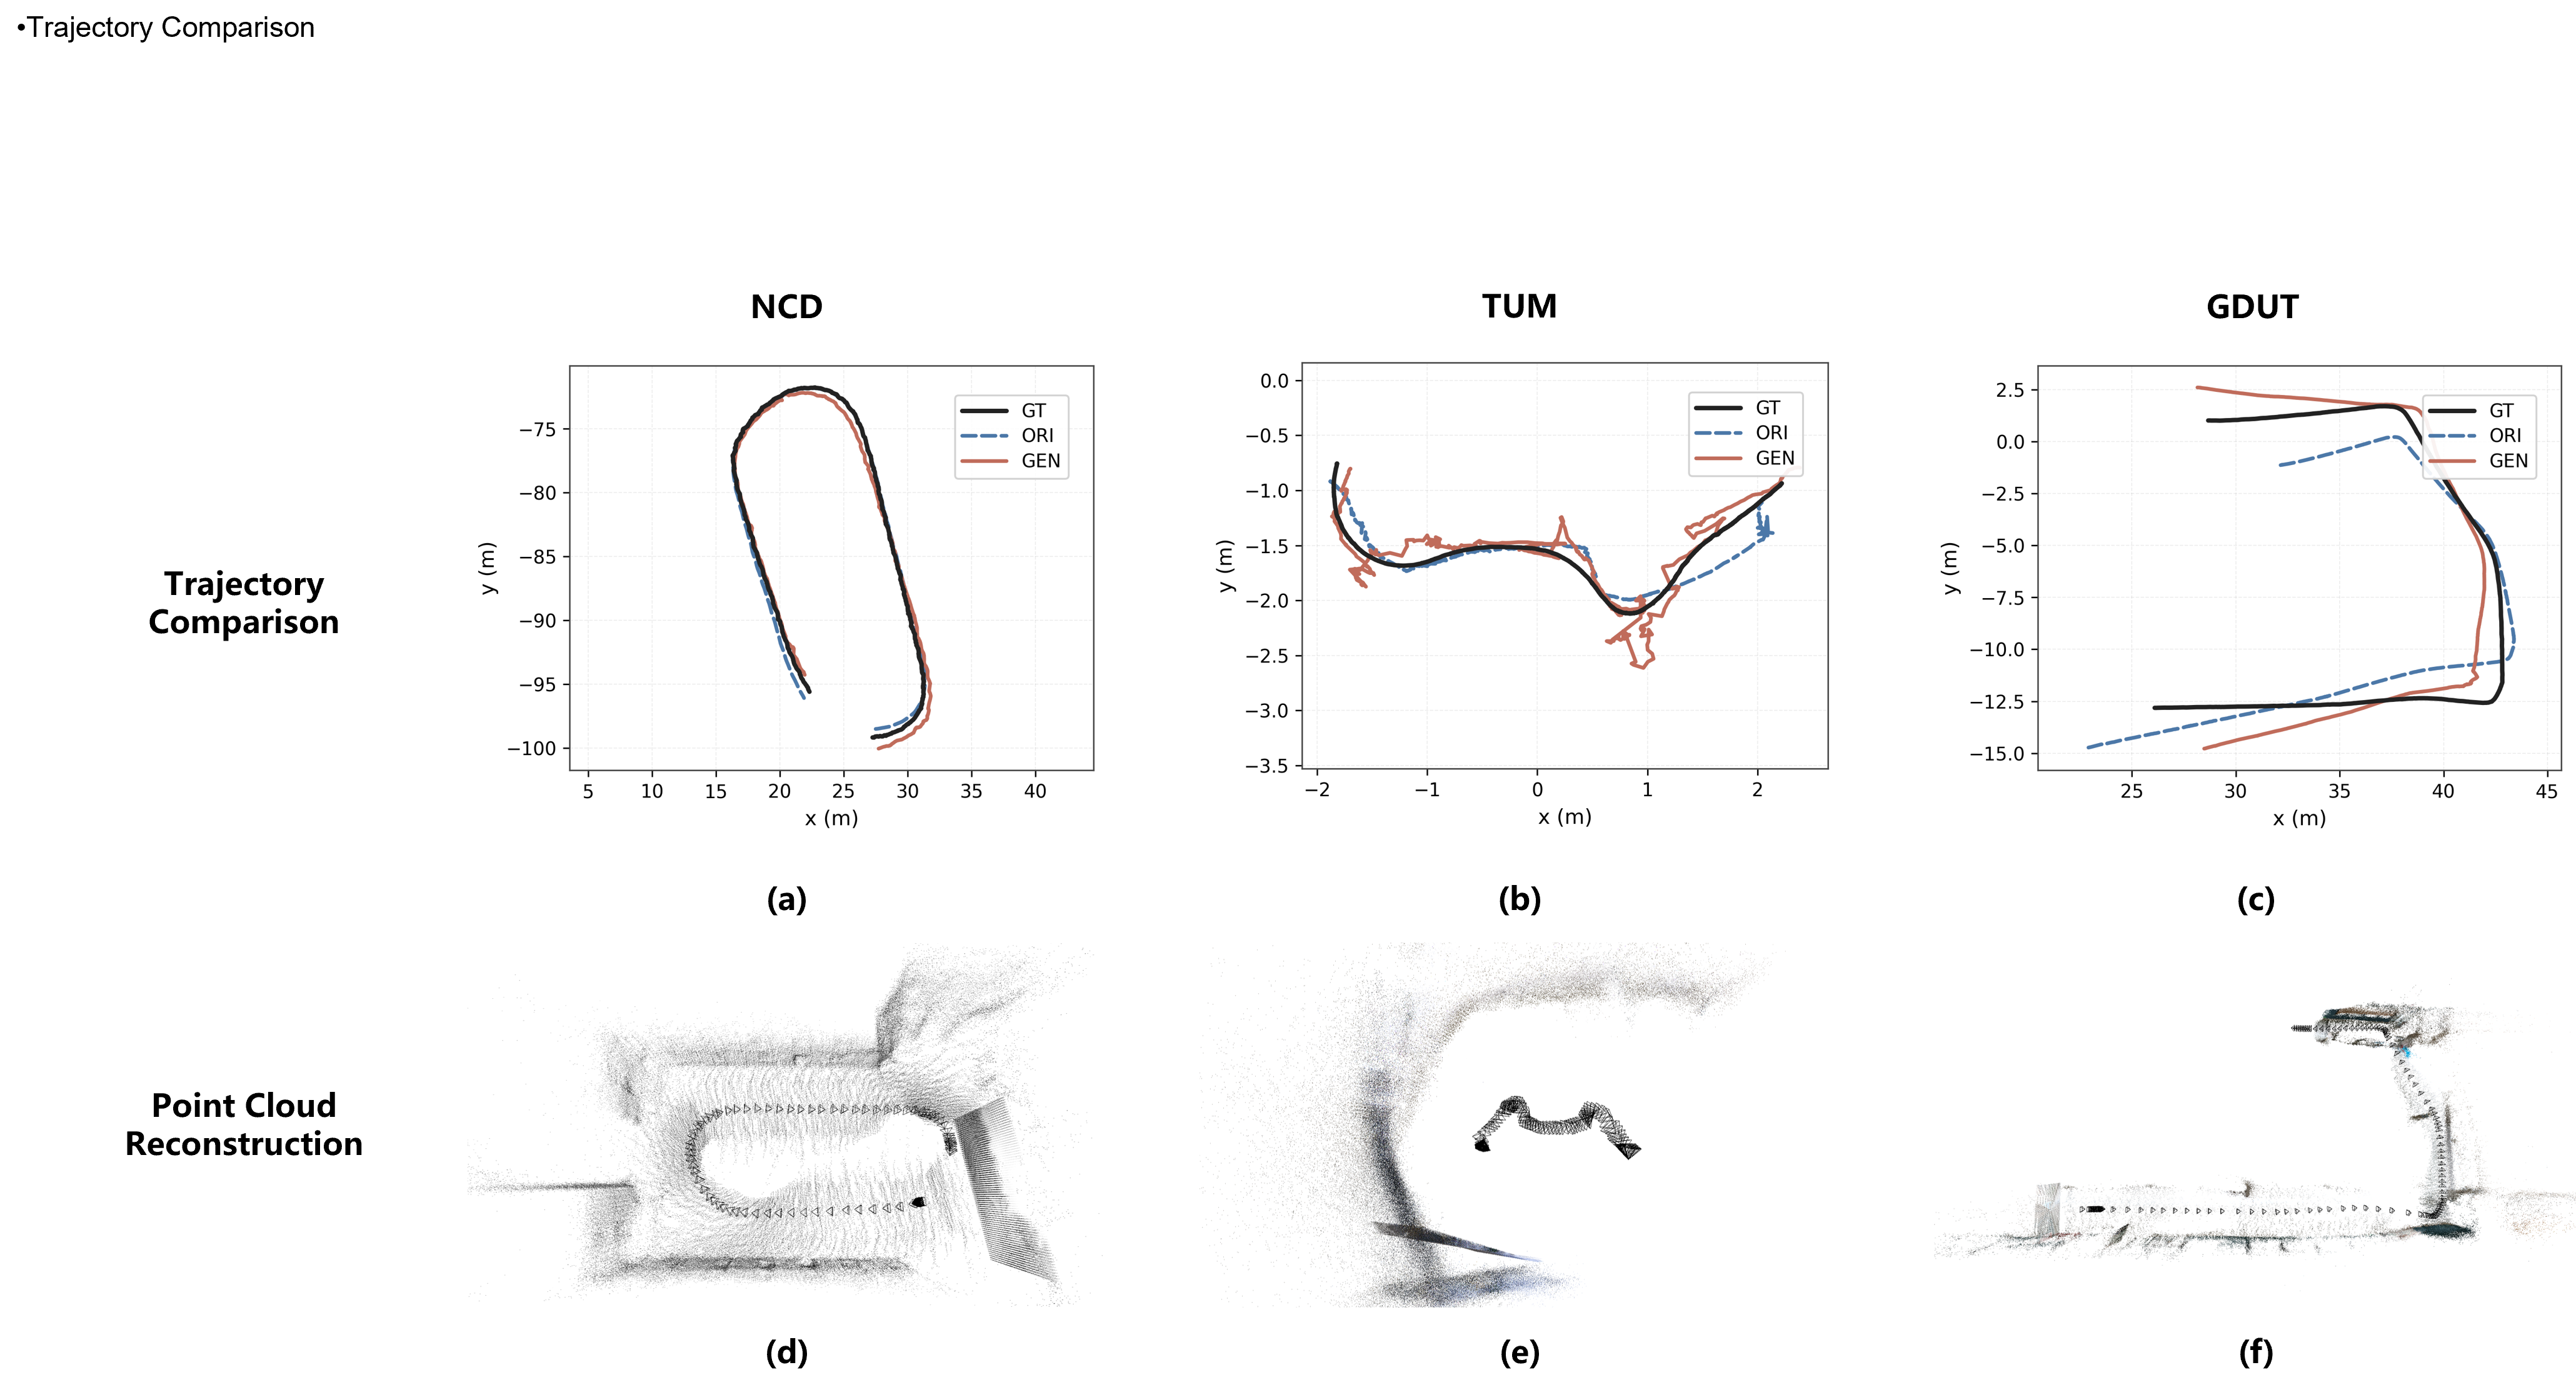
\includegraphics[width=\textwidth]{figures/fig_exp1_trajectory_map.png}
\caption{Trajectory comparison and point-cloud reconstruction results on NCD, TUM, and GDUT.}
\label{fig:trajectory_map}
\end{figure*}

\newpage

Table~\ref{tab:compression_accuracy} reports that, on average, the raw image sequence size is 404.16 MiB, while the transmitted \HVM{} representation is 11.12 MiB. This corresponds to an average data reduction of 96.8\%, indicating that the proposed representation substantially reduces transmitted visual data.

The VSLAM results indicate that this reduction can retain task-usable geometric information. The average ORI APE RMSE is 0.694 m, while the average GEN APE RMSE is 0.707 m. Thus, although GEN APE is close to ORI APE on average, sequence-level differences remain: some generated sequences obtain lower APE than their original counterparts, whereas others obtain higher APE. This behavior is expected because \HVM{} does not aim to reconstruct pixel-identical videos, but to retain enough geometric continuity for downstream VSLAM.

Fig.~\ref{fig:trajectory_map} further illustrates this trend by comparing trajectories and point-cloud reconstructions on NCD, TUM, and GDUT. The generated sequences retain the main route structure and support trackable reconstruction in these examples, which suggests that task-usable geometric continuity can be retained under aggressive transmission reduction.

\subsection{Edge-Side Motion Estimation Benchmark}
\label{subsec:motion_benchmark}

The second experiment compares three edge-side motion estimation choices for constructing motion memory. This benchmark evaluates qualitative segmentation consistency and runtime efficiency, rather than supervised motion-label accuracy.

% This table is included by sections/04_experiments.tex.
\begin{table}[!t]
\renewcommand{\arraystretch}{1.14}
\caption{Runtime comparison of edge-side Motion Response methods.}
\label{tab:motion_benchmark}
\centering
\footnotesize
\setlength{\tabcolsep}{1.5pt}
\begin{tabular*}{\columnwidth}{@{\extracolsep{\fill}}lcccc@{}}
\toprule
Method & Time (s) $\downarrow$ & ms/pair $\downarrow$ & Rel. Cost $\downarrow$ & Valid (\%) $\uparrow$ \\
\midrule
\textbf{Phase Correlation} & \textbf{4.51} & \textbf{4.70} & \textbf{1.00$\times$} & \textbf{100.0} \\
ORB Feature Tracking & 11.73 & 12.22 & 2.60$\times$ & 85.7 \\
Farneback Optical Flow & 29.75 & 30.99 & 6.59$\times$ & 100.0 \\
\bottomrule
\end{tabular*}%
\vspace{0.2em}

\parbox{\columnwidth}{\footnotesize The benchmark is computed on the 40s GDUT clip with 961 frames, corresponding to 960 adjacent frame pairs. Rel. Cost is normalized by PC runtime. Valid ratio denotes the percentage of adjacent frame pairs that produce usable motion evidence.}
\end{table}


\begin{figure*}[!t]
\centering
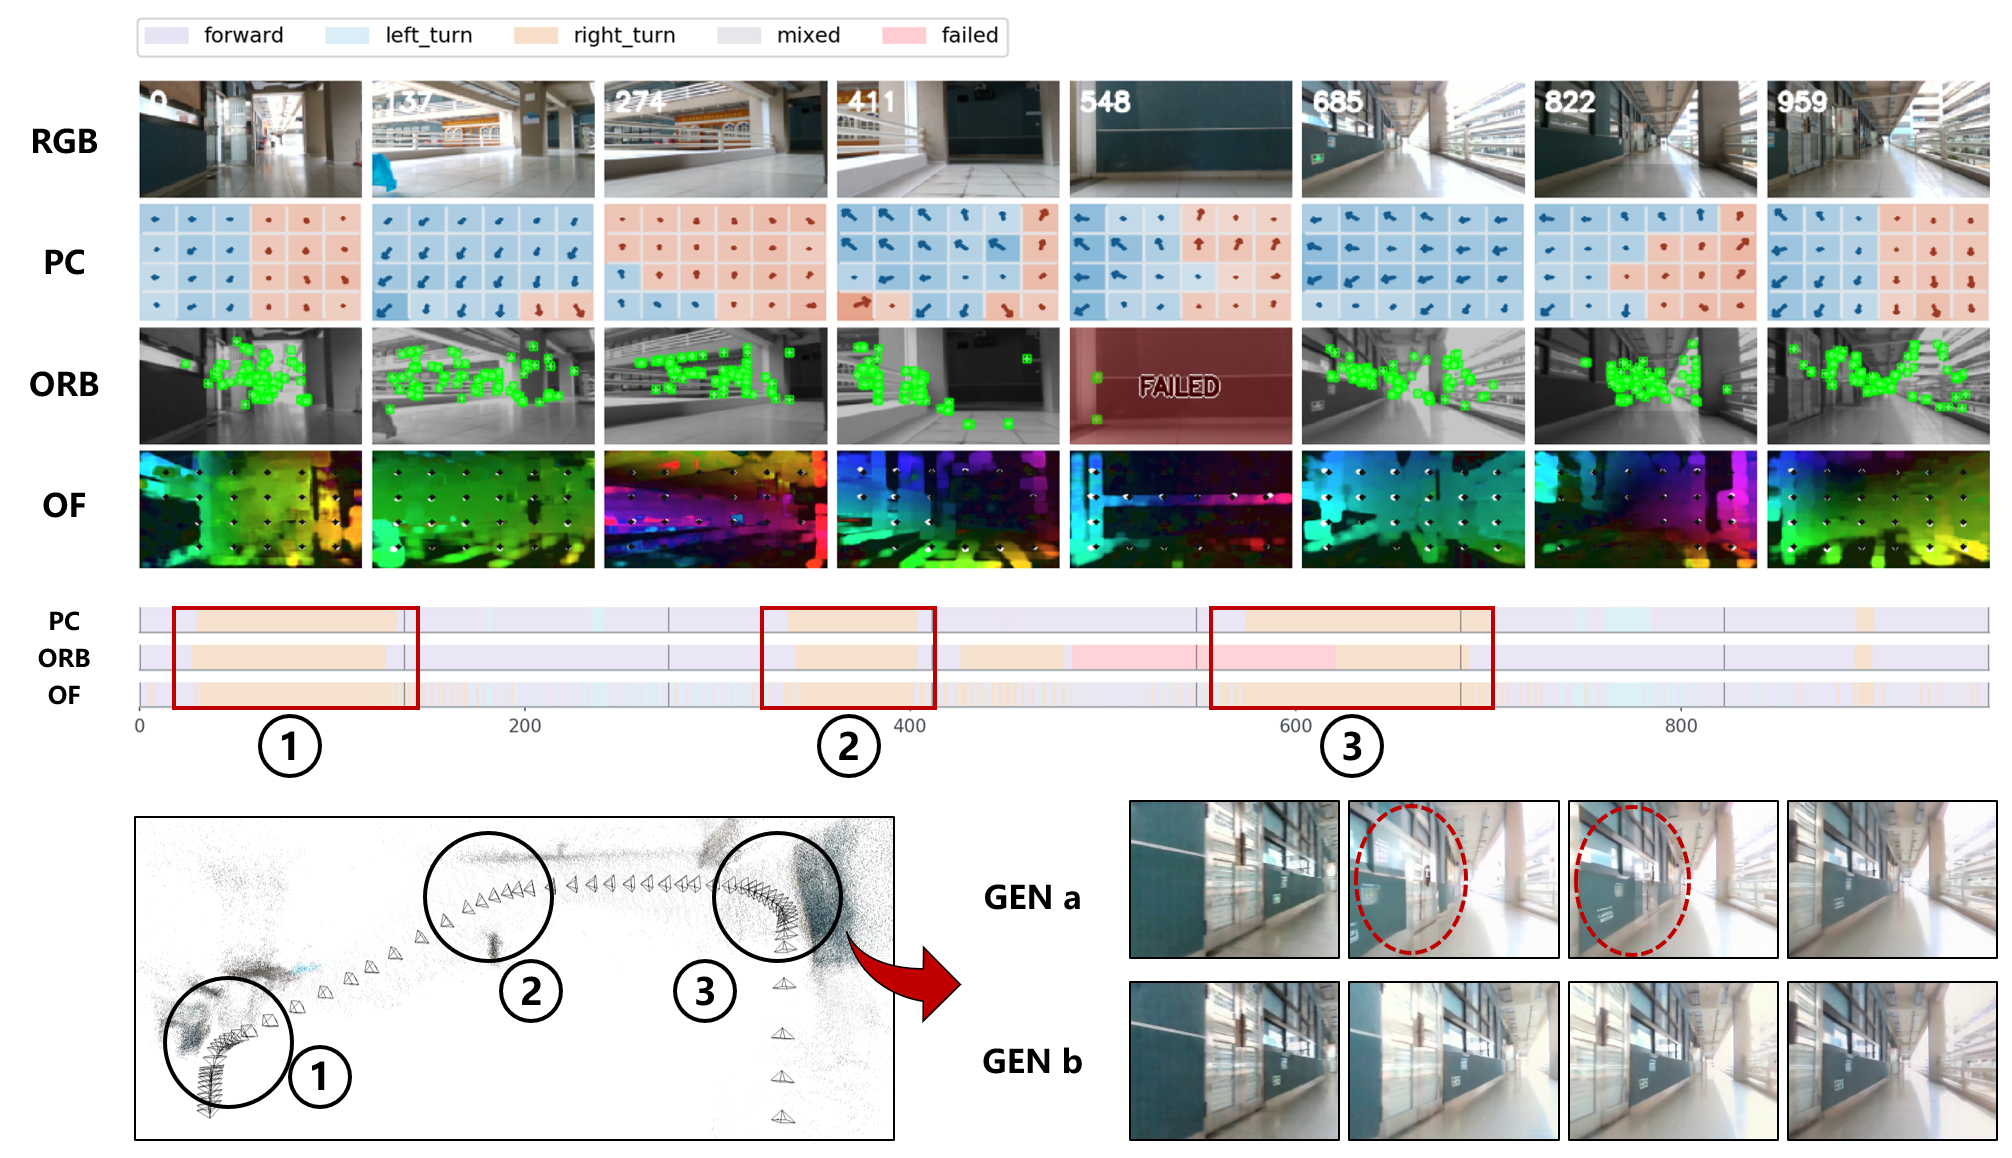
\includegraphics[width=\textwidth]{figures/fig_exp2_motion_benchmark.png}
\caption{Qualitative comparison of phase correlation, ORB feature tracking, and Farneback optical flow for edge-side motion estimation.}
\label{fig:motion_benchmark}
\end{figure*}

\newpage

Fig.~\ref{fig:motion_benchmark} and Table~\ref{tab:motion_benchmark} show the qualitative behavior and runtime cost of the three methods. The valid-output ratio denotes the fraction of frame pairs for which a method produced usable motion evidence.

PC is the lightest option, requiring 4.51 s in total and 4.70 ms per frame pair. ORB feature tracking requires 11.73 s, or 2.60x the PC cost, and produces usable motion evidence for 85.7\% of the evaluated pairs. Farneback optical flow (OF) provides a denser motion field, but its runtime increases to 29.75 s, or 6.59x the PC cost.

These results reflect different edge-side tradeoffs. ORB depends on repeatable local features and can fail in low-texture regions, rapid turns, or tracking-difficult intervals. OF can describe richer local motion but introduces a much higher computational burden. PC provides only coarse global motion, but it can capture language-level trends such as forward motion and turning at the lowest cost, making it suitable as the default edge encoder in \HVM.

\subsection{LoRA Ablation for the World-Model Decoder}
\label{subsec:lora_ablation}

The final experiment ablates the Base and LoRA variants of the world-model decoder.

% This table is included by sections/04_experiments.tex.
\begin{table}[!t]
\renewcommand{\arraystretch}{1.14}
\caption{LoRA ablation results for the world-model decoder.}
\label{tab:lora_ablation}
\centering
\scriptsize
\setlength{\tabcolsep}{2pt}
\begin{tabular*}{\columnwidth}{@{\extracolsep{\fill}}llrrrrr@{}}
\toprule
Data & Dec. & ORI APE & GEN APE & LPIPS & SSIM & FID \\
\midrule
NCD & Base & 0.142 & 0.539 & 0.270 & 0.593 & 50.151 \\
NCD & LoRA & 0.142 & \textbf{0.289} & 0.307 & 0.507 & 23.950 \\
TUM & Base & 0.224 & 0.320 & 0.392 & 0.634 & 71.539 \\
TUM & LoRA & 0.224 & \textbf{0.224} & 0.514 & 0.480 & 104.861 \\
GDUT & Base & 0.354 & 0.968 & 0.345 & 0.587 & 62.169 \\
GDUT & LoRA & 0.354 & \textbf{0.451} & 0.372 & 0.559 & 70.845 \\
Avg. & Base & 0.240 & 0.609 & 0.335 & 0.604 & 61.286 \\
Avg. & LoRA & 0.240 & \textbf{0.321} & 0.398 & 0.515 & 66.552 \\
\bottomrule
\end{tabular*}%
\vspace{0.2em}

\parbox{\columnwidth}{\footnotesize APE values are RMSE in meters. LPIPS, SSIM, and FID are auxiliary image-fidelity metrics and are not the final task-level objective.}
\end{table}


Table~\ref{tab:lora_ablation} shows that the average GEN APE RMSE decreases from 0.609 m with the Base decoder to 0.321 m with LoRA, while the average ORI APE RMSE remains 0.240 m because the original sequences are not affected by the decoder. The same trend appears on NCD, TUM, and GDUT, suggesting that LoRA improves VSLAM-oriented decoding performance across the evaluated data groups.

The image-fidelity metrics do not improve in the same direction. On average, LPIPS changes from 0.335 to 0.398, SSIM changes from 0.604 to 0.515, and FID changes from 61.286 to 66.552. Since LPIPS, SSIM, and FID measure image fidelity and are not the optimization target of \HVM, these changes do not by themselves indicate system failure.

Instead, the ablation indicates that traditional image similarity and VSLAM trajectory quality are not fully aligned in this setting. LoRA appears to bias the decoder toward SLAM-friendly geometry and temporal continuity rather than pixel-level similarity, which supports the task-oriented nature of \HVM.

% !TEX root = ../main.tex

% ==================================================
\section{Discussion and Limitations}
\label{sec:discussion}
% ==================================================

\VLMemCodec{} is designed around efficient visual transmission in Edge--Cloud VSLAM rather than generic video delivery. Its VLMem payload keeps visual anchors and language cues as compact Vision--Language Memory, and the reconstructed sequence is evaluated primarily by downstream VSLAM trajectory quality. This task-driven framing should not be interpreted as a closed-form optimization of the full VSLAM pipeline; instead, it provides a practical coding design whose trajectory quality is assessed through the cloud-side VSLAM estimator.

The results also show that image-fidelity metrics and downstream VSLAM trajectory quality are not fully aligned. LPIPS, SSIM, and FID are useful auxiliary metrics because they characterize complementary aspects of reconstructed image appearance, but they do not necessarily move in the same direction as APE RMSE. In the MGDR ablation, decoder refinement implemented through LoRA-based low-rank increments reduces REC APE in the reported setting, while the auxiliary image-fidelity metrics do not improve uniformly.

The current prototype demonstrates the communication benefit of the compact VLMem payload, but cloud-side world-model reconstruction remains the major runtime bottleneck in the present implementation. This separates the communication benefit from the current reconstruction-runtime bottleneck. The compact transmitted representation reduces payload size, while final end-to-end latency also depends on the world-model decoder, accelerator memory, batching and parallel serving, and inference optimization. The present system should therefore be viewed as a prototype for validating the efficient visual transmission formulation in Edge--Cloud VSLAM, not as a fully real-time optimized cloud service.

The cloud-side world-model decoder also introduces a reconstruction limitation. Although visual anchors and language cues constrain the reconstruction, the reconstructed frames may still contain hallucinations, local geometric inconsistency, viewpoint drift, dynamic-object artifacts, or texture changes. Therefore, reconstructed frames should be treated as task-usable reconstructions for downstream VSLAM evaluation, not physically accurate observations.

The edge-side encoder uses lightweight motion and semantic event cues rather than precise dense motion estimation. Phase correlation provides coarse language-level motion conditions, not full optical flow. Future work will focus on faster world-model serving, model compression or distillation, and parallel reconstruction of VLMem units; stronger geometry-aware constraints, closed-loop SLAM feedback, and uncertainty-aware decoding; and task-specific lightweight decoders for efficient visual transmission in Edge--Cloud VSLAM.

% ==================================================
\section{Conclusion}
\label{sec:conclusion}
% ==================================================

This paper presented \VLMemCodec, a Vision--Language Memory coding framework with world-model reconstruction for efficient visual transmission in Edge--Cloud VSLAM. The proposed framework represents dense image streams as a VLMem payload with visual anchors and language cues, and reconstructs task-usable visual sequences on the cloud using a vision--language conditioned world-model decoder refined through MGDR.

The experimental results show a favorable compression--trajectory tradeoff: the transmitted VLMem payload substantially reduces visual data, REC APE remains close to ORI APE on average, phase correlation provides low-cost motion cues for the edge encoder, and MGDR reduces REC APE in the decoder ablation. The results also indicate that auxiliary image-fidelity metrics are not fully aligned with VSLAM trajectory quality. Future work will further improve geometric consistency and closed-loop VSLAM-aware reconstruction.


% -------------------- Acknowledgment --------------------
\section*{Acknowledgment}
% TODO: Add funding and acknowledgments if needed. Remove this section for anonymous review if required.
The authors would like to thank XXX.

% -------------------- References --------------------
\ifCLASSOPTIONcaptionsoff
  \newpage
\fi

\bibliographystyle{IEEEtran}
\bibliography{references}

% -------------------- Biographies --------------------
% TODO: IEEE biographies are often required in final journal versions, but may be removed during anonymous review.
\begin{IEEEbiographynophoto}{First Author}
Biography text here.
\end{IEEEbiographynophoto}

\begin{IEEEbiographynophoto}{Second Author}
Biography text here.
\end{IEEEbiographynophoto}

\begin{IEEEbiographynophoto}{Third Author}
Biography text here.
\end{IEEEbiographynophoto}

\end{document}
